%%%%%%%%%%%%%%%%%%%%%%%%%%%%%%%%%%%%%%%%%%%%%%%%%%%%%%%%%%%
%% Supporting Information
%% TODO:
%%    TODO: Free energy corrections to OER intermediates, OER mechanism
%%    TODO: Is there any cross-validation happening here? I don't think so
%%%%%%%%%%%%%%%%%%%%%%%%%%%%%%%%%%%%%%%%%%%%%%%%%%%%%%%%%%%


% #########################################################
\section{Active Learning ML Section}  % ###################
% #########################################################
%
% #########################################################
% | - Active Learning ML Section

% %%%%%%%%%%%%%%%%%%%%%%%%%%%%%%%%%%%%%%%%%%%%%%%%%%%%%%%%%
\subsection{Candidate space generation}  % %%%%%%%%%%%%%%%%
% %%%%%%%%%%%%%%%%%%%%%%%%%%%%%%%%%%%%%%%%%%%%%%%%%%%%%%%%%
%
% %%%%%%%%%%%%%%%%%%%%%%%%%%%%%%%%%%%%%%%%%%%%%%%%%%%%%%%%%
% | - Candidate space generation


% ################################# Paragraph #############
% %%%%%%%%%%%%%%%%%%%%%%%%%%%%%%%%%%%%%%%%%%%%%%%%%%%%%%%%%
% Basic intro into candidate generation
% High-level overview again
%   * Data mining OQMD MP fro AB2/3 entries
%   * Reduce data set by eliminating structurally redundant systems
%     * This is done with Ankit's scheme
%   *
% %%%%%%%%%%%%%%%%%%%%%%%%%%%%%%%%%%%%%%%%%%%%%%%%%%%%%%%%%
% | - Paragraph start
%
Here we describe in more detail the methodology to construct the set of structural candidates that were considered.
%
At a high-level, the procedure is to mine materials databases for entries with the desired non-element specific stoicheometry (\latin{i.e.} \ABtwo and \ABthree).
%
Since many of the entries in these databases are structurally redundant with one another,
we used a structure classification scheme to reduce the data set to a structurally unique set.
%
Once this is accomplished, the elements of interest were then substituted into the database structures, which at this point had their original elemental composition from their database.
%
And finally, the structures are isotropically expanded or contracted to accommodate the difference between the atomic radii of the original elements in the structure and the user defined elements.
%
Below we go into more detail for each of these steps.
% __|


% ################################# Paragraph #############
% %%%%%%%%%%%%%%%%%%%%%%%%%%%%%%%%%%%%%%%%%%%%%%%%%%%%%%%%%
% Data-mining OQMD and MP
% %%%%%%%%%%%%%%%%%%%%%%%%%%%%%%%%%%%%%%%%%%%%%%%%%%%%%%%%%
% | - Paragraph start
Herein, we take advantage of the structural diversity already present in materials databases to construct our candidates.
%
We utilized two materials databases, the Open Quantum Materials (OQMD) and the Materials Project (MP) databases because of their large and diverse datasets of crystalline inorganic materials.
%
% TODO Approx. when did Ankit parse these databases
At the time that we originally mined these databases (TEMP 2018? TEMP), there were \num{61471} inorganic compounds in the MP database and \num{435583} entries in the OQMD database.
%
The databases have expanded the number of entries considerably since we originally parsed them, so we'd like to caution the reader that these exact numbers are out of date.
%
Herein, for simplicity we'll refer to the quantitative figures of these databases in the present, instead of past, tense.
%
The structural classification scheme of Jain \latin{et al.} \cite{Jain2018} was then used to classify the structure and element-nonspecific stoicheometry of each structure (\num{497054} in total).
%
% COMBAK Revise if Ankit's scheme becomes it's own section
See section TEMP for more details on the symmetry based structural classification scheme.
%
Once classified, we selected all entries with the desired stoicheometry of \ABtwo and \ABthree,
for which MP has \num{2424} and \num{2341} \ABtwo and \ABthree entries, respectively,
and OQMD has \num{4736} and \num{28,883} \ABtwo and \ABthree entries, respectively.
%
% COMBAK double check, is this the right reason?
The reason that there are considerably more \ABthree compounds in OQMD is due to the extensive compositional permutation of the cubic Perovskite structure (ABO\textsubscript{3} ABO3) with the A cation removed.
%
% TODO
Within each stoicheometry, the structural classification was used to eliminate structurally redundant systems, \latin{i.e.} systems that share their stoicheometry, space-group, and Wyckoff positions.
%
This process reduces the data set to \num{620} and \num{219} unique structures of \ABtwo and \ABthree for MP and \num{397} and \num{194} structurally unique \ABtwo and \ABthree OQMD entries.
%
% COMBAK
Combining the MP and OQMD data sets ultimately results in a dataset of \num{688} \ABtwo and \num{254} \ABthree structurally unique candidates.
%
% __|



% | - Table of OQMD MP Structures
\begin{table}[!htb]

  \caption{\label{table:database_structures}
    %
    (a) Number of entries in the OQMD and MP materials databases for the \ABtwo and \ABthree stoichiometries.
    %
    (b) Final number of unique structural candidates for \ABtwo and \ABthree.
    }
  %
  % | - Subtable a
  \begin{subtable}{.5\linewidth}
  \centering
  \caption{}
  %
   %
    %
    \begin{tabular}{cccc}
    \textbf{}         & \textbf{}        & \multicolumn{2}{c}{\textbf{Entries}} \\
    \textbf{Database} & \textbf{Stoich.} & \textbf{Total}   & \textbf{Unique}   \\
    OQMD              &                  & 61,471           &                   \\
                      & \ABtwo           & 4,736            & 397               \\
                      & \ABthree         & 28,883           & 194               \\
    \hline
    MP                &                  & 435,583          &                   \\
                      & \ABtwo           & 2,424            & 620               \\
                      & \ABthree         & 2,341            & 219
    \end{tabular}
    %
   %
  %
  \end{subtable}
  % __|
  %
  %
  \newline
  \vspace*{0.8 cm}
  \newline
  %
  %
  % | - Subtable b
  \begin{subtable}{.5\linewidth}
  \centering
  \caption{}
  %
   %
    %
    \begin{tabular}{cc}
    \multicolumn{2}{c}{\textbf{Final Candidate Set}} \\
    \textbf{Stoich.}   & \textbf{Unique Structures}  \\
    \ABtwo             & 688                         \\
    \ABthree           & 254
    \end{tabular}
    %
   %
  %
  \end{subtable}
  % __|
  %
\end{table}
% __|


% ################################# Paragraph #############
% %%%%%%%%%%%%%%%%%%%%%%%%%%%%%%%%%%%%%%%%%%%%%%%%%%%%%%%%%
% Structural classification scheme
%
% TODO Should this be its own section?
% Might be a good idea to have Ankit write an overview of the method here
% %%%%%%%%%%%%%%%%%%%%%%%%%%%%%%%%%%%%%%%%%%%%%%%%%%%%%%%%%
% | - Paragraph start
%
This structural classification scheme can directly serve as a structural fingerprint and has successfully been applied towards the prediction of formation energies of inorganic compounds \cite{Jain2018}.
% __|



% ################################# Paragraph #############
% %%%%%%%%%%%%%%%%%%%%%%%%%%%%%%%%%%%%%%%%%%%%%%%%%%%%%%%%%
% Pre-optimization
%
% * We use a simple isotropic expansion/contraction for this paper
% * I also tried Kirsten's more robust pre-optimizer, but had minimal impacts on the results (performance of AL/ML models)
% * Pre-optimization is an important step because it determines how "physical" the structure is, which affects it's fingerprint and ultimately how well the ML surrogate model can learn and predict the energy of these structures
% %%%%%%%%%%%%%%%%%%%%%%%%%%%%%%%%%%%%%%%%%%%%%%%%%%%%%%%%%
% | - Paragraph start
% until all interatomic pair-wise distances are above the summation of the atoms atomic radii.

% __|



% | - __old__
%
% The candidate for \IrOtwo and \IrOthree were generated from existing experimental structures in the OQMD and Materials Project databases by considering only structurally unique systems, where structural uniqueness.
%
% This was done by parsing for structurally unique systems based on the crystal symmetry classification scheme of Ankit.
%
% __|

% __|


% %%%%%%%%%%%%%%%%%%%%%%%%%%%%%%%%%%%%%%%%%%%%%%%%%%%%%%%%%
\subsection{Structure featurization and data processing}  %
% %%%%%%%%%%%%%%%%%%%%%%%%%%%%%%%%%%%%%%%%%%%%%%%%%%%%%%%%%
%
% %%%%%%%%%%%%%%%%%%%%%%%%%%%%%%%%%%%%%%%%%%%%%%%%%%%%%%%%%
% | - Structure featurization and data processing
% TODO Cite Wolverton paper
Structures are featurized using the Voronoi tessellation method developed by TEMP.
%
0-variance features that don't encode for any information within a set of structures with constant composition and stoicheometry are then removed (\num{271} to \num{101} feature columns).
% TODO Add all of the feature engineering steps here
% __|


% %%%%%%%%%%%%%%%%%%%%%%%%%%%%%%%%%%%%%%%%%%%%%%%%%%%%%%%%%
\subsection{Gaussian process regression model}  % %%%%%%%%%
% %%%%%%%%%%%%%%%%%%%%%%%%%%%%%%%%%%%%%%%%%%%%%%%%%%%%%%%%%
% Relevant details about the ML Gaussian process here  % @Chris
%
% %%%%%%%%%%%%%%%%%%%%%%%%%%%%%%%%%%%%%%%%%%%%%%%%%%%%%%%%%
% | - Gaussian process regression model
%
The Gaussian Process model utilized two isotropic Gaussian (RBF) kernels, with one kernel having a larger length scale parameter and the other one having a length scale parameter that operates on shorter length scales.
%
% TODO Double check that I said it correctly, might be minimizing the LML
The hyperparameters of the GP kernel are optimized every time the GP is trained such that the log marginal likelihood of the model and training data is maximized.
%
The initial values of the hyper parameters are as follows:

% | - Table of GP Hyper parameters
\begin{table}[htbp]
\centering
\begin{tabular}{cc}
  GP Hyper Paramter & Initial Value \\
  noise & 0.02542 \\
  sigmaL & 1.0049 \\
  sigmaF & 5.19 \\
  alpha & 0.018
\end{tabular}
\end{table}
% __|

% __|


% %%%%%%%%%%%%%%%%%%%%%%%%%%%%%%%%%%%%%%%%%%%%%%%%%%%%%%%%%
\subsection{Bulk polymorph DFT optimization}  % %%%%%%%%%%%
% %%%%%%%%%%%%%%%%%%%%%%%%%%%%%%%%%%%%%%%%%%%%%%%%%%%%%%%%%
%
% VASP
% PBE exchange correlation functional
% spin-polarized calculations
% plane-wave cutoff of 600 eV
% %%%%%%%%%%%%%%%%%%%%%%%%%%%%%%%%%%%%%%%%%%%%%%%%%%%%%%%%%
% | - Bulk polymorph DFT optimization
%
A variable k-point mesh is used such that a k-point density of at least \num{20} k-points per reciprocal space dimension.
%
All bulk systems were run through the following computational recipe to converge the equilibrium structure.
%
The recipe has \num{3} distinct phases, and structures are only advanced to the next phase when the previous phase completes without error.
%
1. A ISIF \num{7} calculation to optimize only the volume (initial volume of cell may be really off).
%
2. \num{3} consecutive ISIF \num{3} relaxations to fully converge the lattice and atomic positions.
%
3. A final ISIF \num{2}, calculation to relax the atomic coordinates only to avoid errors associated with changing the cell volume with a fixed plane-wave cutoff basis.
%
The final ISIF \num{2} step is run with an electronic energy SCF convergence criteria of \SI{1e-6} eV and the ionic relaxation has a tight force convergence criteria of \SI{1e-3}{\electronvolt\per\angstrom}.
% __|


% %%%%%%%%%%%%%%%%%%%%%%%%%%%%%%%%%%%%%%%%%%%%%%%%%%%%%%%%%
\subsection{Structural coordination motif identification} %
% %%%%%%%%%%%%%%%%%%%%%%%%%%%%%%%%%%%%%%%%%%%%%%%%%%%%%%%%%
%
% %%%%%%%%%%%%%%%%%%%%%%%%%%%%%%%%%%%%%%%%%%%%%%%%%%%%%%%%%
% | - Structural coordination motif identification
Several esoteric structural features were found in the DFT optimized structures and can be categorized as one of two types,
legitimate structural motifs not characterized by the scheme of Waroquiers et. al. \cite{Waroquiers2017}, and arguably non-physical structural artifacts, including:
% TODO Add more of these
- unassociated oxygen atoms
- molecular oxygens in the unit cell
% __|


% __|


% #########################################################
\section{Electrochemical OER Computational Methods}  % ####
% #########################################################
%
% #########################################################
% | - Electrochemical OER Computational Methods


% %%%%%%%%%%%%%%%%%%%%%%%%%%%%%%%%%%%%%%%%%%%%%%%%%%%%%%%%%
\subsection{Density Functional Theory Methods}  % %%%%%%%%%
% %%%%%%%%%%%%%%%%%%%%%%%%%%%%%%%%%%%%%%%%%%%%%%%%%%%%%%%%%
%
% %%%%%%%%%%%%%%%%%%%%%%%%%%%%%%%%%%%%%%%%%%%%%%%%%%%%%%%%%
% | - Density Functional Theory Methods
%
All OER calculations were performed using density functional theory (DFT) implemented via the Vienna \latin{ab-initio} simulation package (VASP)
\cite{Kresse1995,Kresse1996_0,Kresse1996_1}
and utilizing the PBE exchange-correlation functional\cite{Perdew1996}.
%
Dipole corrections were imposed on all non-symmetric slabs to counteract spurious dipole interactions between the periodic cells.\cite{Neugebauer1992}
%
% TODO COMBAK, make this section more general, k-points were treated differently
% for different calculations
A 4x4x3 k-point mesh with gamma-point centered Monkshort-packing\cite{Monkhorst1976} was used for all slabs.
%
The plane-wave energy cutoff was \SI{500}{\electronvolt}.
%
% COMBAK Figure out how much spacing was used for all slabs
All slab calculations maintained a vacuum spacing in between TEMP and \SI{15}{\angstrom}
%
All structures were relaxed with utilizing the conjugate gradient algorithm as implemented in VASP (IBRION\num{=2}).
%
The simulation stop criteria used was that all atoms must satisfy a maximum force threshold of \SI{0.02}{\electronvolt\per\angstrom}.
% __|


% %%%%%%%%%%%%%%%%%%%%%%%%%%%%%%%%%%%%%%%%%%%%%%%%%%%%%%%%%
\subsection{OER Thermodynamic Methodology}  % %%%%%%%%%%%%%
% %%%%%%%%%%%%%%%%%%%%%%%%%%%%%%%%%%%%%%%%%%%%%%%%%%%%%%%%%
%
% %%%%%%%%%%%%%%%%%%%%%%%%%%%%%%%%%%%%%%%%%%%%%%%%%%%%%%%%%
% | - OER Thermodynamic Methodology
%
Here we will outline the procedure used to carry out OER simulations on the various slabs of \IrOtwo and \IrOthree.
%
The procedure was as follows:
%
Stable stoichiometric terminations were cut from the bulk
%
% COMBAK
% TODO Add Vesta reference
Stable termination planes were guesstimated via intuition, and the x-ray diffraction pattern tool from Vesta.
%
Next, electrochemical surface coverage was elucidated via a surface Pourbaix analysis.
%
This elucidates the coverage under operating conditions (> \SI{1.23}{\volt vs. RHE}) for each slab.
%
% COMBAK
Finally we conducted a thermodynamic/limiting potential analysis of the OER mechanistic pathway (Volcano plot, limiting potentials, etc).
% __|


% %%%%%%%%%%%%%%%%%%%%%%%%%%%%%%%%%%%%%%%%%%%%%%%%%%%%%%%%%
\subsection{Simulated XRD Patterns}  % %%%%%%%%%%%%%%%%%%%%
% %%%%%%%%%%%%%%%%%%%%%%%%%%%%%%%%%%%%%%%%%%%%%%%%%%%%%%%%%
%
% %%%%%%%%%%%%%%%%%%%%%%%%%%%%%%%%%%%%%%%%%%%%%%%%%%%%%%%%%
% | - Simulated XRD Patters
%
The simulated XRD spectra for \aIrOthree, \bIrOthree, and \rIrOtwo were computed using the VESTA software package.
% TODO Insert the paramters for the XRD spectra
We used a TEMP wavelength source thing.


% | - Figure | OER Scaling Relations
\begin{figure*}[!htb]
\centering
\makebox[\textwidth][c]{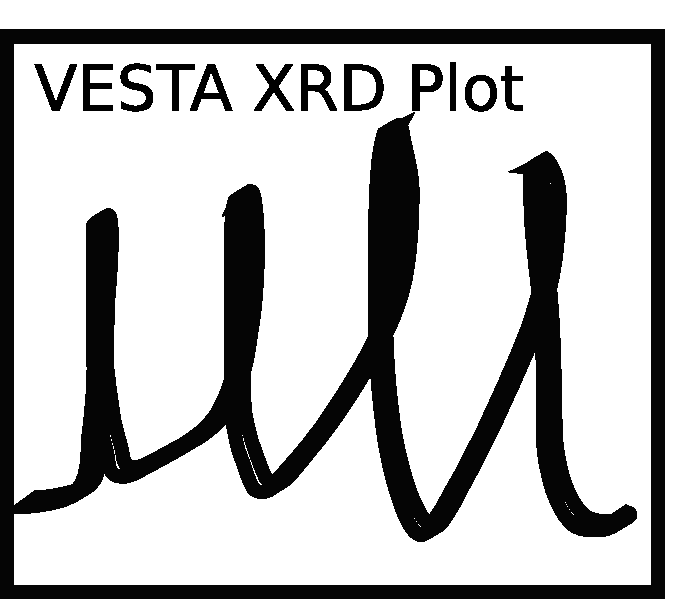
\includegraphics{02_figures/xrd_plots/xrd_plots.pdf}}
\caption{\label{fig:xrd_patterns}
TEMP CAPTION
}
\end{figure*}
% __|


% %%%%%%%%%%%%%%%%%%%%%%%%%%%%%%%%%%%%%%%%%%%%%%%%%%%%%%%%%
\subsection{Surface Energy Pourbaix Methodology}  % %%%%%%%
% %%%%%%%%%%%%%%%%%%%%%%%%%%%%%%%%%%%%%%%%%%%%%%%%%%%%%%%%%
%
% %%%%%%%%%%%%%%%%%%%%%%%%%%%%%%%%%%%%%%%%%%%%%%%%%%%%%%%%%
% | - Surface Energy Pourbaix Methodology
%
Surface energy Pourbaix plots were constructed by calculating the surface energy of each slab by under standard conditions (\si{\volt}\num{=0} and pH\num{=0}) and then utilizing the computational hydrogen electrode (CHE) to compute the potential dependence of the surfaces.
%
Surface energy calculations were performed for various facets for slabs of increasing thickness.
%
% TODO Insert reference for surface E calcs
The bulk energy was then extracted by fitting the total energy of the slabs against the number of layers as explained in TEMP.
%
This was  done to avoid common issues of surface energy divergence associated with using a separate bulk energy calculation.
%
The sensitivity of a given slab to an applied bias is dependent on the composition of the surface,
in particular, the effect of coverage of electrolyte species which can deposit oxygen, hydrogen, and hydroxide species on the surface layers.
%
These additional \ce{O} and \ce{H} atoms are not referenced to the atoms in the slab, but are instead referenced to the computational hydrogen electrode and water-splitting reaction.
%
% TODO Type out equations for surface energy calculation
The equation for is as follows:
% __|


% %%%%%%%%%%%%%%%%%%%%%%%%%%%%%%%%%%%%%%%%%%%%%%%%%%%%%%%%%
\subsection{OER Scaling Relations}  % %%%%%%%%%%%%%%%%%%%%%
% %%%%%%%%%%%%%%%%%%%%%%%%%%%%%%%%%%%%%%%%%%%%%%%%%%%%%%%%%
% TODO We will make a O(2p) vs. O-OH plot showing that this descriptor correlates with oxidation state like that some of the structures are close to ideal
%
% %%%%%%%%%%%%%%%%%%%%%%%%%%%%%%%%%%%%%%%%%%%%%%%%%%%%%%%%%
% %%%%%%%%%%%%%%%%%%%%%%%%%%%%%%%%%%%%%%%%%%%%%%%%%%%%%%%%%
% | - OER Scaling Relations

% ################################# Paragraph #############
% %%%%%%%%%%%%%%%%%%%%%%%%%%%%%%%%%%%%%%%%%%%%%%%%%%%%%%%%%
%
% %%%%%%%%%%%%%%%%%%%%%%%%%%%%%%%%%%%%%%%%%%%%%%%%%%%%%%%%%
Figure~\ref{fig:scaling_relations} shows the scaling relations between the adsorption free energies of the OER intermediate species for the studied \IrOx slabs.
%
It can be seen clearly that the data points corresponding to the three \IrOthree polymorphs are roughly \SI{1}{\electronvolt} weaker binding than the \rIrOtwo points.
%
This generally weaker binding of the \IrOthree stoichiometry is responsible for the observed improvement in theoretical activity.
%
The \DGOOH vs.\DGOH relationship is very close to the traditional ``universal scaling relations'', demonstrating that our materials do not break the infamous \DGOOH vs. \DGOH scaling.


% | - Figure | OER Scaling Relations
\begin{figure*}[!htb]
\centering
% \makebox[\textwidth][c]{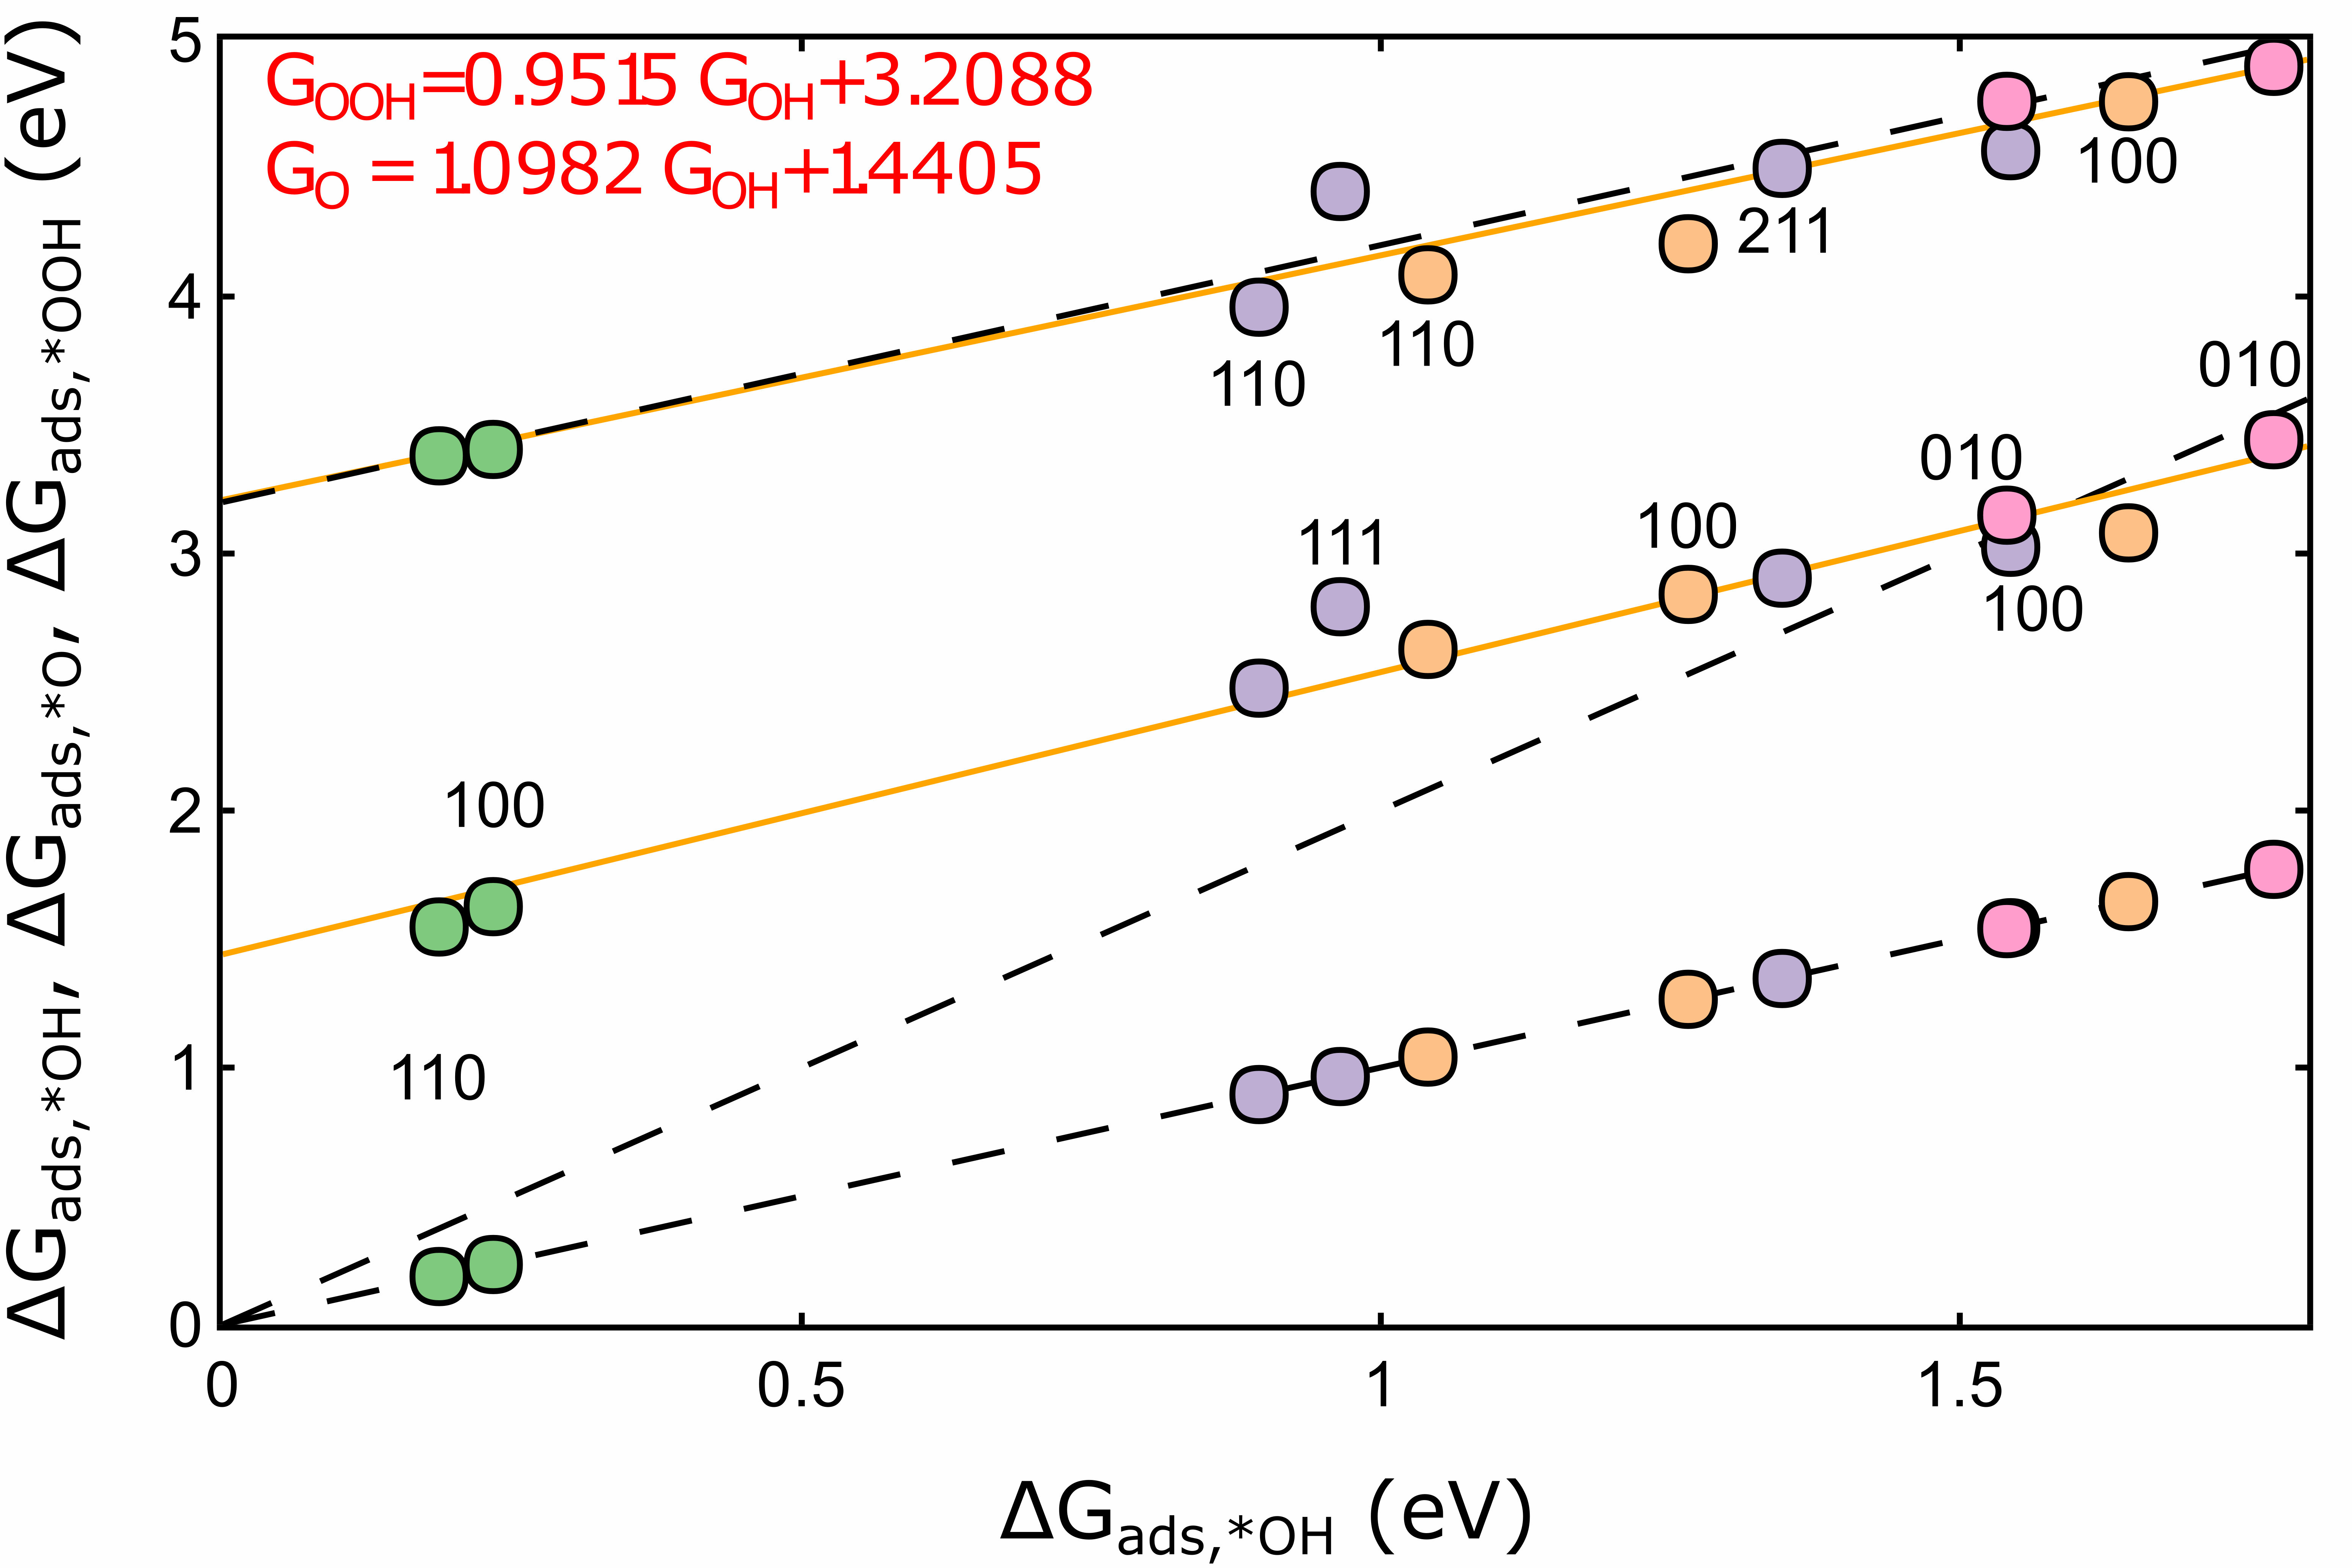
\includegraphics{02_figures/oer_activity_stability/00_master__oer_scaling__main_v0__outplot2.png}}
\makebox[\textwidth][c]{\includegraphics{02_figures/oer_activity_stability/oer_scaling.pdf}}
\caption{\label{fig:scaling_relations}
Relationship between the adsorption free energies of the three key OER intermediates (*OH, *O, *OOH), with \DGOH chosen as the dependent variable.
%
Best fit lines are provided for \DGOOH vs. \DGOH and \DGO vs. \DGOH.
%
Additionally, ``universal scaling relations'' for \DGOOH vs. \DGOH and \DGO vs. \DGOH are shown (black dotted lines) to emphasize our deviation from the traditionally reported scaling fits.
%
The \DGOH line is  shown as guide to eye.
% TODO Do I have to redefine the color convention every caption?
}
\end{figure*}
% __|

% __|


% %%%%%%%%%%%%%%%%%%%%%%%%%%%%%%%%%%%%%%%%%%%%%%%%%%%%%%%%%
\subsection{Bulk Systems}  % %%%%%%%%%%%%%%%%%%%%%%%%%%%%%%
% %%%%%%%%%%%%%%%%%%%%%%%%%%%%%%%%%%%%%%%%%%%%%%%%%%%%%%%%%
%
% %%%%%%%%%%%%%%%%%%%%%%%%%%%%%%%%%%%%%%%%%%%%%%%%%%%%%%%%%
% %%%%%%%%%%%%%%%%%%%%%%%%%%%%%%%%%%%%%%%%%%%%%%%%%%%%%%%%%
% | - Bulk Systems
% Formation energies of 4 polymorphs

% __|


% %%%%%%%%%%%%%%%%%%%%%%%%%%%%%%%%%%%%%%%%%%%%%%%%%%%%%%%%%
\subsection{Table of OER energetics}  % %%%%%%%%%%%%%%%%%%%
% %%%%%%%%%%%%%%%%%%%%%%%%%%%%%%%%%%%%%%%%%%%%%%%%%%%%%%%%%
%
% %%%%%%%%%%%%%%%%%%%%%%%%%%%%%%%%%%%%%%%%%%%%%%%%%%%%%%%%%
% %%%%%%%%%%%%%%%%%%%%%%%%%%%%%%%%%%%%%%%%%%%%%%%%%%%%%%%%%
% | - Table of OER energetics

\begin{table}[!htb]

  \caption{\label{table:oer_table}
    %
    (a) TEMP
    }
  %
  % | - Subtable a
  \begin{subtable}{.5\linewidth}
  \centering
  \caption{}
  %
   %
    %
    \begin{tabular}{cccc}
    \textbf{}         & \textbf{}        & \multicolumn{2}{c}{\textbf{Entries}} \\
    \textbf{Database} & \textbf{Stoich.} & \textbf{Total}   & \textbf{Unique}   \\
    OQMD              &                  & 61,471           &                   \\
                      & \ABtwo           & 4,736            & 397               \\
                      & \ABthree         & 28,883           & 194               \\
    \hline
    MP                &                  & 435,583          &                   \\
                      & \ABtwo           & 2,424            & 620               \\
                      & \ABthree         & 2,341            & 219
    \end{tabular}
    %
   %
  %
  \end{subtable}
  % __|
  %
  %
  \newline
  \vspace*{0.8 cm}
  \newline
  %
  %
  % | - Subtable b
  \begin{subtable}{.5\linewidth}
  \centering
  \caption{}
  %
   %
    %
    \begin{tabular}{cc}
    \multicolumn{2}{c}{\textbf{Final Candidate Set}} \\
    \textbf{Stoich.}   & \textbf{Unique Structures}  \\
    \ABtwo             & 688                         \\
    \ABthree           & 254
    \end{tabular}
    %
   %
  %
  \end{subtable}
  % __|
  %
\end{table}
% __|



% __|
